%
% PROTOCOL DESCRIPTION
%
\JWlone{Protocol Description} \label{sec:protocol-description}

\begin{JWfunc}%
  {\JWfuncSymOPE}%
  {The ideal $\JWfieldGeneral{}$-OPE functionality \JWfuncSymOPE{}}%
  {fig:func-ope}

  Parametrized by a finite field size $q$ and maximal polynomial degree $k$.

  \begin{JWfuncSteps}

  \item Upon receiving input $a \in \mathbb{F}_q^k$ from \JWpOne{}, verify that
    there is no stored input from \JWpOne{}, yet; else ignore that input. Next
    record $a$ and send \JWmsgTwo{processing}{\JWpOne{}} to the adversary.

  \item Upon receiving input $x \in \mathbb{F}_q$ from \JWpTwo{}, verify that
    there is no stored input from \JWpTwo{}, yet; else ignore that input. Next
    record $x$ and send \JWmsgTwo{processing}{\JWpTwo{}} to the adversary.

  \item Upon receiving a message \JWmsgTwo{delivery}{\JWpTwo{}} from the
    adversary, verify that \JWpTwo{} and \JWpOne{} have both already provided
    some input; else ignore that message. Next, compute $y \leftarrow
    \sum_{i=1}^k a_ix^i$ and send $y$ to \JWpTwo{}.

  \end{JWfuncSteps}
\end{JWfunc}

\begin{JWboxed}%
  {Graphical Representation of \JWfuncSymOPE}%
  {fig:graph-ope}

  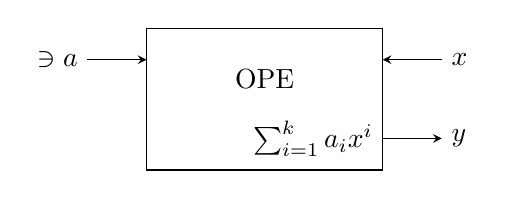
\begin{tikzpicture}[>=stealth]

    \node (OPE) at (8.5,0) {OPE};
    \draw (OPE) +(-1.5,-1.15) rectangle +(1.5,0.65);

    \draw [<-] (OPE) ++(-1.5,0.25) node [anchor=west] {} -- +(-0.75,0) node
    [anchor=east] {$\JWfieldGeneral \ni a$};

    \draw [<-] (OPE) ++(1.5,0.25) node [anchor=east] {} -- +(0.75,0) node
    [anchor=west] {$x$};

    \draw [->] (OPE) ++(1.5,-0.75) node [anchor=east] {$\sum_{i=1}^k a_ix^i$}
    -- +(0.75,0)
    node [anchor=west] {$y$};

  \end{tikzpicture}
\end{JWboxed}

\begin{JWprotocol}%
  {\JWprotoSymOPE}%
  {Protocol: Oblivious Polynomial Evaluation}%
  {fig:proto-ope}

  \JWprotoPhase{Setup:}

  \begin{JWprotoSteps}

  \item \JWpOne{} generates OAFEs and EDs (see section \ref{sec:prep-eval})

  \item \JWpOne{} sends the OAFEs and EDs to \JWpTwo{}

  \end{JWprotoSteps}


  \JWprotoPhase{Evaluation:}

  \begin{JWprotoSteps}

  \item Upon receiving the OAFEs and EDs, \JWpTwo{} evaluates the EDs one by one
    and saved the values needed for further computations

  \item After the Evaluation, \JWpTwo{} adds the values of the last two EDs and
    queries a special last OAFE with that value. The then received new value is
    the result of the computation $y = \sum_{i=1}^k a_ix^i$.

  \end{JWprotoSteps}

\end{JWprotocol}
